%%%%%%%% ICML 2022 EXAMPLE LATEX SUBMISSION FILE %%%%%%%%%%%%%%%%%

\documentclass[nohyperref]{article}

% Recommended, but optional, packages for figures and better typesetting:
\usepackage{microtype}
\usepackage{graphicx}
\usepackage{subfigure}
\usepackage{booktabs} % for professional tables

% hyperref makes hyperlinks in the resulting PDF.
% If your build breaks (sometimes temporarily if a hyperlink spans a page)
% please comment out the following usepackage line and replace
% \usepackage{icml2022} with \usepackage[nohyperref]{icml2022} above.
\usepackage{hyperref}


% Attempt to make hyperref and algorithmic work together better:
\newcommand{\theHalgorithm}{\arabic{algorithm}}

% Use the following line for the initial blind version submitted for review:
\usepackage{icml2022}

% If accepted, instead use the following line for the camera-ready submission:
%\usepackage[accepted]{icml2022}

% For theorems and such
\usepackage{amsmath}
\usepackage{amssymb}
\usepackage{mathtools}
\usepackage{amsthm}

% if you use cleveref..
\usepackage[capitalize,noabbrev]{cleveref}

%%%%%%%%%%%%%%%%%%%%%%%%%%%%%%%%
% THEOREMS
%%%%%%%%%%%%%%%%%%%%%%%%%%%%%%%%
\theoremstyle{plain}
\newtheorem{theorem}{Theorem}[section]
\newtheorem{proposition}[theorem]{Proposition}
\newtheorem{lemma}[theorem]{Lemma}
\newtheorem{corollary}[theorem]{Corollary}
\theoremstyle{definition}
\newtheorem{definition}[theorem]{Definition}
\newtheorem{assumption}[theorem]{Assumption}
\theoremstyle{remark}
\newtheorem{remark}[theorem]{Remark}

% Todonotes is useful during development; simply uncomment the next line
%    and comment out the line below the next line to turn off comments
%\usepackage[disable,textsize=tiny]{todonotes}
\usepackage[textsize=tiny]{todonotes}


% The \icmltitle you define below is probably too long as a header.
% Therefore, a short form for the running title is supplied here:
\icmltitlerunning{Submission and Formatting Instructions for ICML 2022}

\begin{document}

\twocolumn[
\icmltitle{Unified Maximizing Q-Learning and Behavior Cloning for Offline RL}

% It is OKAY to include author information, even for blind
% submissions: the style file will automatically remove it for you
% unless you've provided the [accepted] option to the icml2022
% package.

% List of affiliations: The first argument should be a (short)
% identifier you will use later to specify author affiliations
% Academic affiliations should list Department, University, City, Region, Country
% Industry affiliations should list Company, City, Region, Country

% You can specify symbols, otherwise they are numbered in order.
% Ideally, you should not use this facility. Affiliations will be numbered
% in order of appearance and this is the preferred way.
\icmlsetsymbol{equal}{*}

\begin{icmlauthorlist}
\icmlauthor{Firstname1 Lastname1}{equal,yyy}
\icmlauthor{Firstname2 Lastname2}{equal,yyy,comp}
\icmlauthor{Firstname3 Lastname3}{comp}
\icmlauthor{Firstname4 Lastname4}{sch}
\icmlauthor{Firstname5 Lastname5}{yyy}
\icmlauthor{Firstname6 Lastname6}{sch,yyy,comp}
\icmlauthor{Firstname7 Lastname7}{comp}
%\icmlauthor{}{sch}
\icmlauthor{Firstname8 Lastname8}{sch}
\icmlauthor{Firstname8 Lastname8}{yyy,comp}
%\icmlauthor{}{sch}
%\icmlauthor{}{sch}
\end{icmlauthorlist}

\icmlaffiliation{yyy}{Department of XXX, University of YYY, Location, Country}
\icmlaffiliation{comp}{Company Name, Location, Country}
\icmlaffiliation{sch}{School of ZZZ, Institute of WWW, Location, Country}

\icmlcorrespondingauthor{Firstname1 Lastname1}{first1.last1@xxx.edu}
\icmlcorrespondingauthor{Firstname2 Lastname2}{first2.last2@www.uk}

% You may provide any keywords that you
% find helpful for describing your paper; these are used to populate
% the "keywords" metadata in the PDF but will not be shown in the document
\icmlkeywords{Machine Learning, ICML}

\vskip 0.3in
]

% this must go after the closing bracket ] following \twocolumn[ ...

% This command actually creates the footnote in the first column
% listing the affiliations and the copyright notice.
% The command takes one argument, which is text to display at the start of the footnote.
% The \icmlEqualContribution command is standard text for equal contribution.
% Remove it (just {}) if you do not need this facility.

%\printAffiliationsAndNotice{}  % leave blank if no need to mention equal contribution
\printAffiliationsAndNotice{\icmlEqualContribution} % otherwise use the standard text.

\begin{abstract}
Offline RL aims to improve target policy based on pre-collected datasets. A major problem of offline RL is the distribution shift, The behavioral cloning algorithms try to constrain the target policy to be close to the offline data. Though this constraint can reduce extrapolation error of out-of-distribution actions, but it will make the learned policy to be conservative. The maximizing Q-Learning algorithms try to learn a perfect Q-value function according to Bellman eqution, then optimize the policy to generate better action to maximize the Q-value function. 
In this work, we unify maximizing Q-learning and behavioral cloning by implicit and explicit way to leverage their advantages. For implicit way, we propose to constrain the generated actions to be close to offline data by GAN; For explicit way, we first map the states to actions in offline data, then we propose multiple importance sampling to learning a weight for different state-action pairs.

It’s more problematic under high-dimension continuous action space, where the offline data only cover a small part of action space.
In this work, we firstly propose multiple importance sampling to better fit the offline data and stabilize the learning process based on DICE. After obtaining the importance weight from aforementioned step, we propose to use latent variables to extract the target policy. Our latent variables based method replaces traditional behavioral cloning methods that map states to actions directly by neural networks. We conducted extensive experiments on the D4RL dataset and use tSNE to visualize the actions generated by out latent variables method. Experiment results show out method improves the cumulative returns and exploration ability simultaneously compared to standard policy extraction algorithms, especially on the high-dimension action space, such as Adroit [1] of D4RL dataset, which makes a well trade-off between exploitation and exploration.

\end{abstract}

\section{Introduction}
\label{submission}

Offline reinforcement learning has wide applications where online interactions with real environment is costly or dangerous, such as autonomous driving and medical experiments. We can only train our model based on prior data. But this poses a major problem that the learned agent tends to be a copy of the behavior of prior data. Existing algorithms all amount to this principle. The regularization-type algorithms measure the discrepancy between target policy and behavioral policy, trying to make them close to each other. The value regularization algorithms, such as pessimistic, try to avoid distribution shift by regularizing the action value function, assigning low values to unobserved actions, and high values to observed actions in offline data. This kind of algorithms will face severe problems in high dimension domains, where observed actions occupy a small part of the action space. The regularization algorithms make the agent very conservative, performing similar actions to offline data in certain states. 
In this work, we propose to use latent variables based on VAE and GAN to map states to actions. Different from traditional methods that map states to actions explicitly by neural networks. The VAE-type latent variable method maps state to a latent variable and then map the latent variable to state, which is similar to encoder-decoder architecture. At the same time, there will be a constraint, such as f-divergence, to make the latent variable follow standard normal distribution, which aims to make the encoder mapping correctly. The GAN-type latent variable method replaces the constraint by a generator and a discriminator. The discriminator tries to discriminate the latent variable and samples from standard normal distribution, while the generator tries to generate more plausible latent variables to fool the discriminator. By introducing this intermediary latent variable, experimental results show it improves the returns greatly, especially in high dimensional occasions. What’s more, we demonstrate by tSNE that it improves the diversity of the generated actions, which is important for offline RL. The intermediary latent variables make the agent less dependent on the trajectories seen on offline data. 

On the other hand, existing algorithms assume the offline data is homogeneous. But in practical, the data may be collected under various sceneries and follows diverse distributions. Some data may be a mixture of human demonstration or hand-designed controllers, the data has different level of optimality. What’s more, it’s also possible that the data is non-Markovian, which is impossible to represent the data using Markovian policy. Such as human demonstrations that depends on external knowledge. Although such data is collected, but when training, our agent doesn’t know the external human knowledge, making it hard to fit behavioral policy. When we use importance sampling algorithms, it’s hard to estimate the distribution of behavioral data, resulting biased estimation of importance weight. 

reminiscent of KL divergence 

For suboptimal or random trajectories, if we fit the offline data by behavioral cloning without using importance sampling, the learned target policy would also be suboptimal or random. 

Considering the suboptimality and diversity of offline data, we propose multiple importance sampling to model the offline data to improve over the behavioral policy. 



\section{Methodology}
We unify the maximizing Q-Learning with behavioral cloning in implicit way and explicit way. Without behavioral cloning, the policy will be wildly extrapolated on unseen actions. In addition, the Q-value function is penalized by uncertainty, for state-action pairs with high uncertainty, their Q values are smaller than those with low uncertainty, thus prompting a pessimistic policy against OOD actions. The behavioral cloning is weighted by advantage of the action, for actions with low advantage, their contributions to the objective will be down-weighted. 

The performance of maximizing Q-Learning depends on how accurate the Q value estimator is. But we only have limited state-action observations, which incurs extrapolation errors from OOD data, especially for continuous action space. This makes the Q value estimator fall easily into suboptimal area.

Behavioral cloning also has its shortcoming. When the offline data form behavioral policy is biased, the target policy we learned is also biased. This means behavioral cloning methods depend heavily on the quality of training data.
\subsection{Implicit Unification}
For the implicit unification, the maximizing Q-Learning is unified with behavioral cloning by adverisally training. In particular, the actions generated by target policy are forced to be close to actions supported by offline data by generative adversarial networks\cite{gan}.  The behavioral cloning item favors generating actions supported by the offline data. At first, we need to learn the Q-value function, which is an ensemble of multiple Q networks penalized by uncertainty.
\begin{equation}
\label{bellman}
Q_{\phi_i}(s,a) =r+\gamma( \underset{1\le j\le N}{\min}Q_{\phi _{j}^{'}}(s',a') -\log \pi _{\theta}( a'|s' )) 
\end{equation}
where $N$ is ensemble size, $\phi _{j}$ and ${\phi _{j}^{'}}$ are parameters of $j$-th Q function and target Q function, $\log \pi _{\theta}( a'|s')$ is the entropy regularization from SAC\cite{sac}. 
The final Q-value would be the minimum of ensemble Q-values, which encourages pessimistic and mitigates over-estimation  for out-of-distribution (OOD) actions. This pessimistic principle can also be seen as uncertainty penalization\cite{edac} where the Q-value of unstable state-action pairs with large variance would be penalized to have smaller values. 
\begin{equation}
\label{pessimism}
E[\underset{1\le j\le N}{\min}Q_{\phi_{j}^{'}}(s,a)] \approx \mu(s,a) -\varPhi ^{-1}( \frac{N-\pi /8}{N-\pi /4+1}) \sigma(s,a) 
\end{equation}
For the policy, an extra loss is introduced to enforce the generated actions to stay close to behavioral policy, this method is called behavioral cloning. The motivation of behavioral cloning is trying to mitigate over-estimation of OOD actions. The policy keeps conservative when generating new actions. The discriminator $D$ loss is
\begin{equation}
\label{gan_d_loss}
\mathcal{L}_{D}=\underset{a \sim p_{data}}{E}[ D(a)] -\underset{\hat{a} \sim \pi _{\theta}(s)}{E}[ D(\hat{a})]
\end{equation}
Policy objective for implicit way is 
\begin{equation}
\begin{aligned}
\label{policy_loss_gan}
\mathcal{L(\pi)}=& \lambda \left[\log \pi_{\theta}(\hat{a}|s) -\underset{1\le j\le N}{\min}Q_{\phi _j}( s,\hat{a}) \right] \\
                 &+ (1-\lambda)E_{\hat{a}\sim \pi_{\theta}( s)}[D(\hat{a})] 
\end{aligned}
\end{equation}
where $\hat{a}=\pi_{\theta}(s)$, $\lambda$ is used to control the degree of conservatism. 
%where $\lambda$ is the uncertainty penalization coefficient. 
%$$ \lambda =\underset{1\le j\le N}{\text{mean}}Q_{\phi _j}( s,\hat{a}) -\underset{1\le j\le N}{\min}Q_{\phi _j}(s,\hat{a}) \approx {\sigma } $$

\textbf{Policy Optimization} The discriminator $D$ tries its best to discriminate the actions from offline data and actions generated by policy. Whiel the policy can be seen as the generator of GAN. The policy optimizater only optimizes parameters of generator and tries to generate actions to fool the discriminator, i.e., generating actions that can't be distinguished by discriminator. Different from mapping states to actions directly, this kind of adversarial training implicitly enforce generated actions to keep close to offline data, so we call it \textbf{Im}plicit \textbf{B}ehavioral \textbf{C}loning (\textbf{ImBC}). At the same time, assuming we have learned a perfect Q-value estimator, maximizing the lower bound $\underset{1\le j\le N}{\min}Q_{\phi _j}(s,\hat{a})$ will force the policy to generate optimal action $\hat{a}$ under state $s$.The entropy regularization
Therefore, the unification leverages the merits of maximizing Q-Learning and behavioral cloning.

\textbf{Q Optimization} In the policy loss, the policy parameters $\pi_{\theta}$ are optimized to maximize the Q value $Q_{\phi}(s, \pi_{\theta}(s))$ without modifying the parameters ${\phi}$ of Q networks. In order to guide the update of policy parameters ${\theta}$, the Q function should be accurate to estimate the Q value for $(s,a)$ pair. In theory, $Q(s,a)$ function is perfect when it can predict the cumulative reward of real environment when performing action $a$ under state $s$. The parameters of Q function are optimized by the observed offline data. To prevent the Q function wildly extrapolated on unseen state-action pairs, we use the pessimistic mechanism to penalize the Q value of state-action pair with high uncertainty, as is shown in \eqref{bellman}. State-action pair with high uncertainty will have lower Q value, as is shown in \eqref{pessimism}. Pessimistic mechanism is especially important for continuous space, where the observed data occupies a small percentage compared with unseen data. Pessimistic mechanism has been adopted by prior works\cite{cql, edac}.

In formula \eqref{policy_loss_gan}, considering the gradient of $
\frac{\partial Q}{\partial \theta}=\frac{\partial Q}{\partial \hat{a}}\frac{\partial \hat{a}}{\partial \theta}
$, to prevent the $\frac{\partial Q}{\partial \hat{a}}$ to dominate gradient, we add a regularization item $\left| \frac{\partial Q}{\partial \hat{a}} \right|^2$ in the loss to force it small, thus making $\frac{\partial \hat{a}}{\partial \theta}$ to dominate the gradient, so as to better optimize the policy parameters $\theta$. The training objective for Q networks would be
\begin{equation}
\begin{aligned}
\label{Q_loss}
& \left(r+\gamma ( \underset{1\le j\le N}{\min}Q_{\phi _{j}^{'}}( s',a') -\log \pi _{\theta}( a'|s') ) - Q_{\phi _i}(s,a) \right)^2  \\  &+ \left| \frac{\partial Q}{\partial \hat{a}} \right|^2
\end{aligned}
\end{equation}


\begin{algorithm}[tb]
   \caption{Unified Maximizing Q-Learning with Implicit BC}
   \label{alg:ImBC}
\begin{algorithmic}
   %\STATE {\bfseries Input:} data $x_i$, size $m$
   \REPEAT
   \STATE Sample mini-batch data ($s,a,r,s\prime$) from $\mathcal{D}$
   \FOR{$i$ {\bfseries to} $n$ time steps}
   \STATE Train $Q$ with \eqref{Q_loss}
   \STATE Train discriminator $D$ with \eqref{gan_d_loss}
   \STATE Train policy with \eqref{policy_loss_gan}
   \ENDFOR
   \UNTIL{converge}
\end{algorithmic}
\end{algorithm}


\subsection{Explicit Way}

For explicit way, we combine maximizing Q-Learning with a weighted neural network that maps states to actions in offline data directly. Different state-action pair will have different weight $w(s,a)$. The weight $w(s,a)$ is learned via multiple importance sampling. We want to maximize the cumulative reward on target policy, simultaneously constrain target policy to be close to behavioral policy. For the weighted behavioral cloning, we use following framework,
\begin{equation}
\label{base_eq}
\underset{d^{\pi}}{\max} E_{(s,a)\sim d^{\pi}}\left[ R( s,a) \right] - \alpha D_f(d^{\pi}||d^D) 
\end{equation}
\begin{equation}
\label{constraint}
s.t.\ \sum_a^{}{d^{\pi}(s,a)}=(1-\gamma) \mu _0+\gamma \mathcal{T}_*d(s), \ \forall s\in S
\end{equation}

where $D_f(d^{\pi}||d^D)$ is $f$-divergence between $d^{\pi}$ and $d^D$, $f$ is convex; $\mathcal{T}_*d(s)=\sum_{\bar{s},\bar{a}}{T(s|\bar{s},\bar{a}) d(\bar{s},\bar{a})}$; The constraint equation \eqref{constraint} makes sure that $d^{\pi}(s,a)$ is the occupancy distribution of the target policy. The frist item in \eqref{base_eq} maximize reward on target policy $\pi(a|s)$, while the second item in \eqref{base_eq} constrain target policy to be close to behavioral policy. The $\alpha$ controls the strength of the constraint.
We reformulate \eqref{base_eq} and \eqref{constraint} by a Lagrangian multiplier $V(s)$:
%\begin{equation}
\begin{flalign}
\label{base_con}
\underset{d^{\pi}}{\max}\ \underset{V\left( s \right)}{\min}E_{s,a \sim d^{\pi}}[R(s,a)] -\alpha D_f(d^{\pi}||d^D) \nonumber \\+\sum_s{V(s) \left( (1-\gamma) \mu _0+\gamma T_*d(s) -\sum_a^{}{d^{\pi}( s,a)} \right)} 
\end{flalign}
%\end{equation}
Note that $\mathcal{T}_*$ is adjoint of $\mathcal{T}$, we have,
$$
\sum_s{V(s) \cdot \mathcal{T}_* d( s)}=\sum_{s,a}{d( s,a) \mathcal{T}V(s,a)}
$$
So
\begin{equation}
\begin{aligned}
&E_{s,a \sim d^{\pi}}[R(s,a)] -\alpha D_f(d^{\pi}||d^D)  \\
&+\sum_s{V(s) ( (1-\gamma) \mu _0+\gamma \mathcal{T}_*d(s) -\sum_a^{}{d^{\pi}( s,a)} )} \\
=& E_{s,a \sim d^{\pi}}[R(s,a)] -\alpha E_{s,a~d^D}[ f( \frac{d^{\pi}(s,a)}{d^D(s,a)} )] \\ 
&+E_{s,a~d^{\pi}}[ \gamma \mathcal{T}V( s,a ) -V(s)] +( 1-\gamma) E_{s \sim \mu _0}[ V(s)] \\
=& E_{s,a \sim d^D}[ \frac{d^{\pi}(s,a)}{d^D(s,a)}A(s,a) -\alpha f( \frac{d^{\pi}(s,a)}{d^D(s,a)})] \\ 
&+(1-\gamma) E_{s \sim \mu _0}[V(s)] \label{eq4}
\end{aligned}
\end{equation}

where $A(s,a)=R(s,a)+\gamma \mathcal{T}V( s,a ) -V(s)$ is the advantage.

Since in real world, the offline data is complicated, we assume the data is heterogeneous. Therefore, we propose multiple importance sampling for the optimization of target policy. The behavioral policy is heterogeneous, so the corresponding target policy should also be heterogeneous. Assuming there are $K$ distributions ($d^{\pi_1}, d^{\pi_2}...d^{\pi_K}$) for target policy, each $d^{\pi_k}$ has coefficient $\beta_k$ its own Q-value and V-value function to fit. Then \eqref{eq4} would become 

\begin{equation}
\begin{aligned}
%\label{mis_bc}
E_{s,a \sim d^D} &\left[ \sum_{k=1}^K{\left( \frac{\beta _kd^{\pi _k}}{d^D}A_k( s,a ) -\alpha \beta _kf( \frac{d^{\pi _k}}{d^D} ) \right)} \right] \\
&+( 1-\gamma) \sum_{k=1}^K{\beta _kE_{s \sim \mu _0}[ V_k( s)]}  \\
=E_{s,a \sim d^D} &\left[ \sum_{k=1}^K{\left( \beta _k\omega _kA_k( s,a) -\alpha \beta _kf( \omega _k ) \right)} \right] \\
&+( 1-\gamma) \sum_{k=1}^K{\beta _kE_{s \sim \mu _0}[ V_k( s)]}   \label{eq_mis_bc}
\end{aligned}
\end{equation}
where $A_k(s,a)=R(s,a)+\gamma \mathcal{T}V_k( s,a ) -V_k(s)$, and $\omega _k = \frac{d^{\pi _k}(s,a)}{d^D(s,a)}$.
When we maximize \eqref{eq_mis_bc}, it is easy to get a closed-form for $\omega _k$, 
\begin{equation}
\label{weight}
\omega _k = (f')^{-1}\left(\frac{A_k( s,a)}{\alpha} \right) =f^{\prime}_{\ast}\left( \frac{A_k(s,a)}{\alpha} \right) 
\end{equation}

Finally, the overall weight is the mean of weights $w_1, w_2, ...w_K$.
We will use this weight to differentially optimize different state-action pairs from the offline data. The \eqref{eq_mis_bc} would become 
\begin{equation}
\label{bc_w_loss}
E_{(s,a) \sim d^D}\left[ \sum_{k=1}^K{\beta _kf_*\left( A_k(s,a) /\alpha \right)} \right] +(1-\gamma) \sum_{k=1}^K{\beta _kE_{s~\mu _0}\left[ V_k(s) \right]}
\end{equation}

The motivation for multiple importance sampling is that if the original data (behavior policy $d^D$) is heterogeneous and follows multiple distributions, then the target policy $d^{\pi}$ should also follow multiple distributions. What’s more, multiple target policies allow the agent to perform multiple optimal actions under similar state s, which is the usual case in practice.

\textbf{Policy Extraction}
The Policy Extraction module is weighted by the weight we learned from \eqref{weight}. 
\begin{equation}
\label{policy_extract}
\underset{\theta}{\max}\underset{( s,a ) \sim d^{\pi}}{E}\log \pi _{\theta}(a|s) =\underset{\theta}{\max}\underset{(s,a) \sim d^D}{E}[ w(s,a) \log \pi _{\theta}(a|s)] 
\end{equation}
where $w(s,a) =\frac{1}{K}\sum_{k=1}^K{w_k}$. For each state-action pair, there would be a specific weight $w(s,a)$, this weight has nothing to do with policy parameter $\theta$, $w(s,a)$ controls the gradient to the policy loss. In \eqref{weight}, for state-action pair that has large advantage, it will get a larger weight, thus contributing more to the gradient; For state-action pair that has small or negative advantage, it will contribute less to the gradient. 

The policy objective for explicit way is 
\begin{equation}
\begin{aligned}
\label{policy_loss_bc}
\mathcal{L(\pi)}=& \lambda \left[\log \pi _{\theta}\left( \hat{a}|s \right) -\underset{1\le j\le N}{\min}Q_{\phi _j}(s,\hat{a}) \right] \\
                 &+ (1-\lambda) w(s,a) \log \pi_{\theta}(a|s) 
\end{aligned}
\end{equation}
where $\lambda$ is the same as \eqref{policy_loss_gan}.
Different from the implicit behavioral cloning in \eqref{policy_loss_gan}, here we map states to actions directly, and assign different weights to different state-action pairs, so as to better optimize the objective for different state-action pairs.


\begin{algorithm}[tb]
   \caption{Unified Maximizing Q-Learning with Explicit BC}
   \label{alg:ImBC}
\begin{algorithmic}
   %\STATE {\bfseries Input:} data $x_i$, size $m$
   \REPEAT
   \STATE Sample mini-batch data ($s,a,r,s\prime$) from $\mathcal{D}$
   \FOR{$i$ {\bfseries to} $n$ time steps}
   \STATE Train $Q$ with \eqref{Q_loss}
   \STATE Train weight $D$ with \eqref{bc_w_loss}
   \STATE Train policy with \eqref{policy_loss_bc}
   \ENDFOR
   \UNTIL{converge}
\end{algorithmic}
\end{algorithm}

\section{Experiments}
We evaluate our proposed approaches against existing approaches on the D4RL benchmark\cite{d4rl} with various continuous environments. For the MUJOCO data, since we evaluate on the v2 version, some methods that are early developed, like CQL, BCQ, may not be comparable with this approach. Implementation details are in the appendix. Similar to previous literatures, we use the normalized average rewards as the evaluating metric. The average rewards are obtained from 10 runs in each evaluation. 

\subsection{Performance on MuJoCo dataset}
The MuJoCo data consists three environments (halfcheetah, hopper, walker2d), each environment consists 5 types (expert, medium-expert, medium-replay, medium, random). In particular, the \textit{expert} data means the 
The \textit{medium} data contains 1M samples generated from early-stoping SAC\cite{sac} policy, where the samples are collected before the policy reaches optimal. The \textit{expert} data contains samples from fully trained online SAC policy. The \textit{medium-expert} means mixing equal amount samples of medium and expert policy. The \textit{medium-replay} contains samples from the replay buffer when the policy reaches medium level. The \textit{full-replay} contains samples from replay buffer of expert policy. The \textit{random} contains samples of random policy.


\textbf{Baselines} We compare out approach with following baselines: EDAC\cite{edac}, which belongs to the maximizing Q learning method, it adopts ensemble-diversified actor-critic to minimize the pairwise alignment (cosine distance) of the gradients for every pair Q-ensemble with regard to actions, thus reducing the ensemble size of Q function. 
IQL\cite{iql}, which belongs to pure behavioral cloning methods; IQL uses a state value function $V(s^{\prime})$ to replace $Q(s^{\prime},a^{\prime})$ to learn the Q function, thus avoiding querying OOD action $a^{\prime}$, then it extracts target policy via advantage-weighted behavioral cloning.
RORL\cite{rorl}, an updated EDAC with noise, making the policy more robust.

Experiment results of our approach and prior baselines are in Table \ref{result-mujoco}. It can be seen our approach \textbf{ImBC} outperforms pure maximizing Q learning method EDAC and pure behavioral cloning method IQL across random to expert data. The performance gap is larger in the expert data, which can be interpreted in that the quality of expert data is higher so behavioral cloning may play an important role for these data compared with pure maximizing Q learning methods. The performance of ImBC and ExBC is different for different domain. For halfcheetah and walker2d, ImBC performs better than ExBC; For hopper data, ExBC performs better. The interpretation might be that hopper data suffers from misestimation due to distributional shift more than halfcheetah and walker2d. Since ExBC has stronger constraint on the generated actions of policy, thus suffering less from distributional shift of actions.

We also investigate the effect of behavioral cloning item in ImBC and ExBC. Figure \ref{fig} shows the results of different $\lambda$ in \eqref{policy_loss_gan} and \eqref{policy_loss_bc}. It can be seen that the performance varies with regard to different $\lambda$. With larger $\lambda$, the agent have stronger constraint to force the policy to generate actions close to offline data. 

Our ImBC can be seen as a combination of these two strategies. 

As for the overall perforance, we surpass prior methods

Experiment results are shown in Table \ref{result-mujoco}. 


\subsection{Performance on Adroit dataset}


\subsection{Ablation Experiments}
The unified maximizing Q-learning and behavioral cloning makes the training converge faster and has better performance compared with only behavioral cloning or maximizing Q-learning. 
We show the behavioral cloning item is necessary for the performance by running ImBC and ExBC with various $\lambda$. When $\lambda = 1$, the algorithm degrades into pure maximizing Q value. When $\lambda = 0$ in \eqref{policy_loss_gan} and \eqref{policy_loss_bc}, the algorithm degrades into pure behavioral cloning. The hyperparameter $\lambda$ can be seen as the degree of conservatism. Larger $\lambda$ means the agent is more conservative. The results in Figure \ref{} show 


\begin{figure*}[htbp]
  \centering
  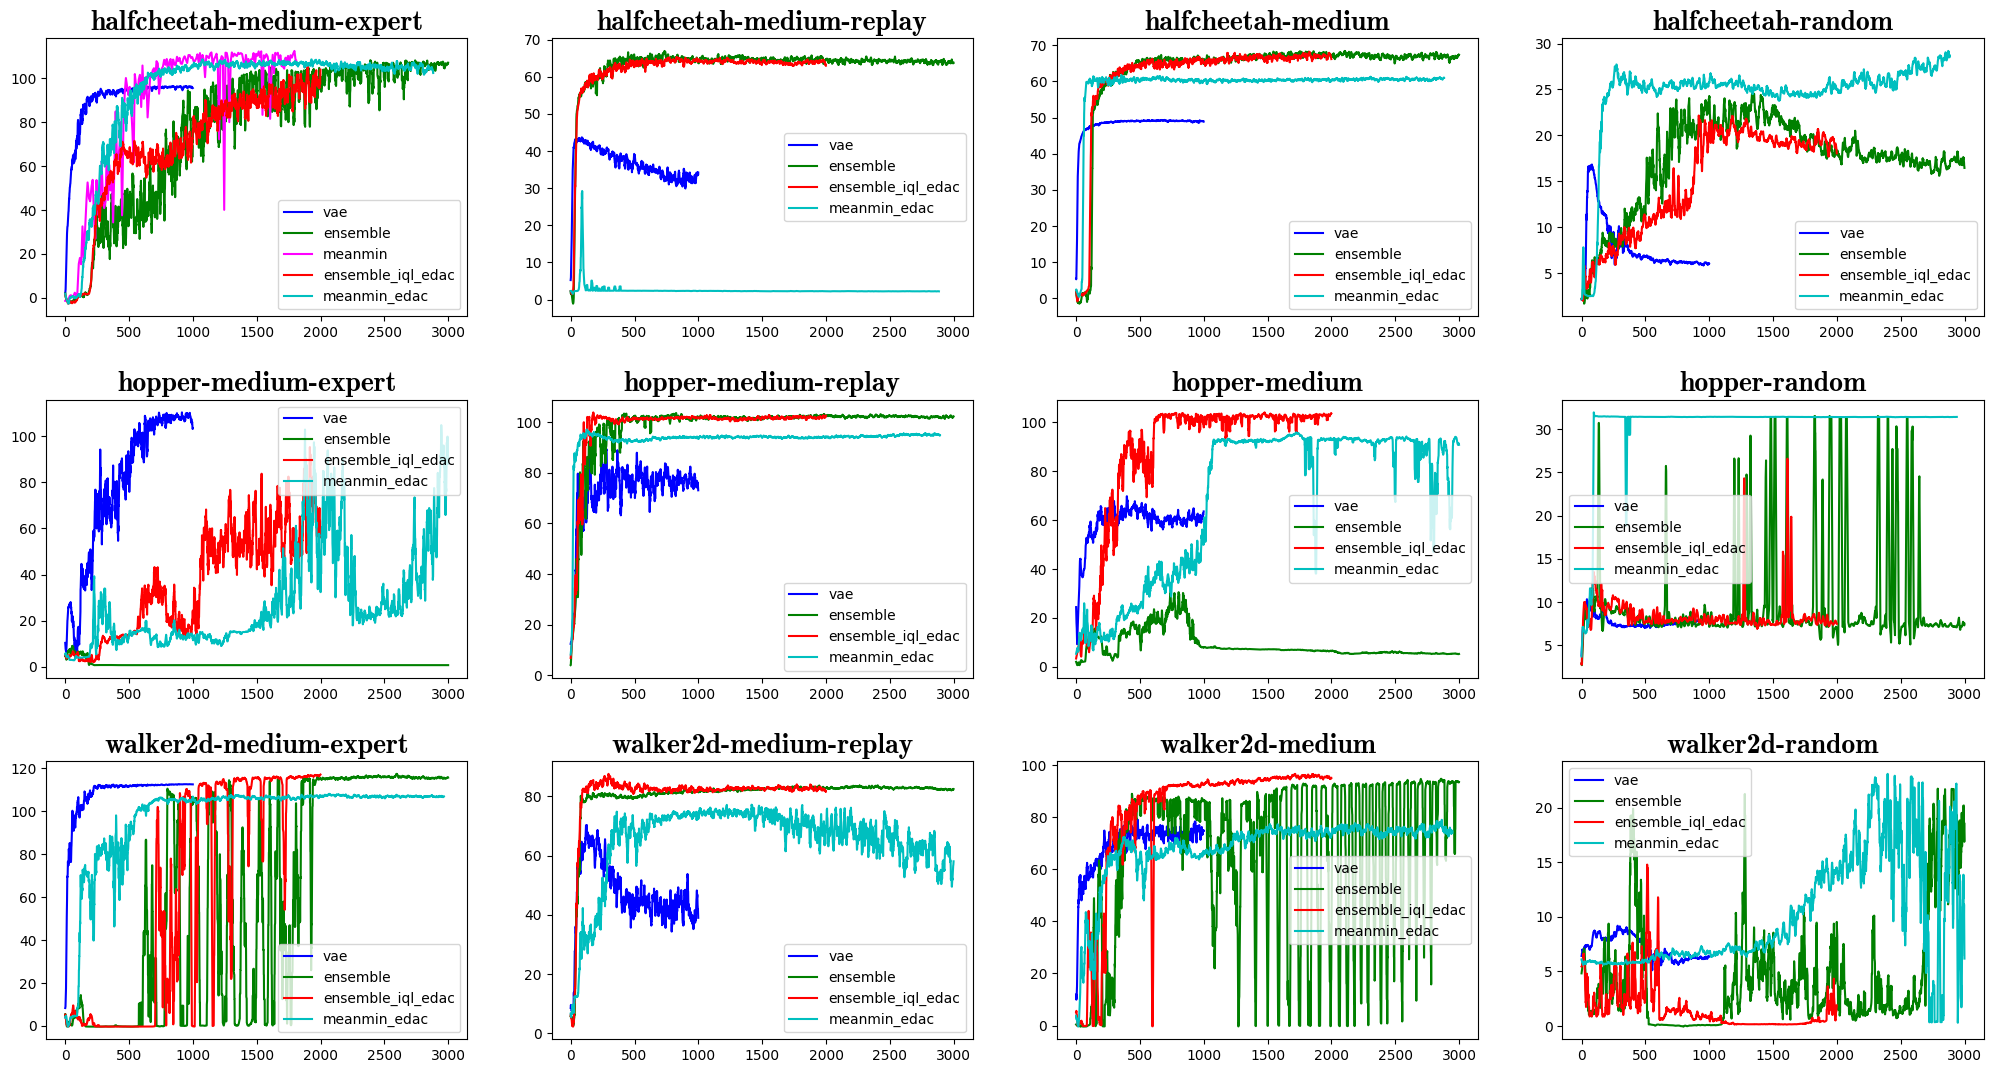
\includegraphics[width=0.99\textwidth]{converge.png}
  \caption{The performance and convergence speed of unified maximizing Q-learning and behavioral cloning}
  \label{fig:conv_speed}
\end{figure*}

\subsection{Visualization of Implicit/Explicit Behavioral Cloning }



\begin{table*}[t]
\caption{Comparison of our method to prior methods.}
\label{result-mujoco}
\vskip 0.15in
\begin{center}
\begin{small}
\begin{tabular}{l|ccccc|cr}
\toprule
Task Name & CQL & ATAC & IQL & EDAC & RORL & ImBC & ExBC \\
\midrule
halfcheetah-medium-expert    & 95.9$\pm$ 0.2& 95.5$\pm$ 0& 86.7$\pm$ 5.3&  106.3$\pm$ 1.9&  107.8$\pm$ 1.1& \bf{113.0$\pm$ 0.4}& 96.7$\pm$ 0.2 \\
halfcheetah-medium-replay    & 83.3$\pm$ 0.6& 49.5$\pm$ 0& 44.2$\pm$ 1.2&  61.3$\pm$ 1.9&  61.9$\pm$ 1.5& \bf{64.0$\pm$ 0.2}& 96.7$\pm$ 0.2 \\
halfcheetah-medium           & 61.9$\pm$ 1.4& 54.3$\pm$ 0& 47.4$\pm$ 0.2&  65.9$\pm$ 0.6&  66.8$\pm$ 0.7& \bf 72.0$\pm$ 0.3& 96.7$\pm$ 0.2 \\
halfcheetah-random           & 74.8$\pm$ 0.5& 4.8$\pm$ 0&  - &             28.4$\pm$ 1.0&  28.5$\pm$ 0.8& \bf 30.0$\pm$ 0.2& 96.7$\pm$ 0.2 \\
\midrule
hopper-medium-expert         & 73.3$\pm$ 0.9& 112.6$\pm$ 0& 91.5$\pm$ 14.3&  110.7$\pm$ 0.1&  112.7$\pm$ 0.2& 90.7$\pm$ 0.2& \bf 112.1$\pm$ 0.3 \\
hopper-medium-replay         & 67.1$\pm$ 0.6& 102.8$\pm$ 0& 94.7$\pm$ 8.6&  101.0$\pm$ 0.5&  102.8$\pm$ 0.5& 104.5$\pm$ 0.1&  103.6$\pm$ 0.2 \\
hopper-medium             & 67.1$\pm$ 0.6&    102.8$\pm$ 0&  66.2$\pm$ 5.7&  101.6$\pm$ 0.6&  104.8$\pm$ 0.1&  58.0$\pm$ 0.2& 65.7$\pm$ 0.2 \\
hopper-random             & 67.1$\pm$ 0.6&    31.8$\pm$ 0&  - &             25.3$\pm$ 10.4&  31.4$\pm$ 0.1&  32.1$\pm$ 1.6& 10.8$\pm$ 0.2\\
\midrule
walker2d-medium-expert     & 73.3$\pm$ 0.9&  116.3$\pm$ 0&  109.6$\pm$ 1.0&  114.7$\pm$ 0.9&  121.2$\pm$ 1.5&  118.0$\pm$ 0.2& 112.2$\pm$ 0.8\\
walker2d-medium-replay      & 67.1$\pm$ 0.6& 94.1$\pm$ 0& 73.8$\pm$ 7.1&  87.1$\pm$ 2.3&  90.4$\pm$ 0.5&  88.0$\pm$ 0.2& \bf95.1$\pm$ 0.4 \\
walker2d-medium            & 67.1$\pm$ 0.6&  91.0$\pm$ 0& 78.3$\pm$ 8.7&  92.5$\pm$ 0.8&  102.4$\pm$ 1.4&  100.0$\pm$ 0.2& 96.7$\pm$ 0.2 \\
walker2d-random            & 67.1$\pm$ 0.6&  8.0$\pm$ 0& - &             16.6$\pm$ 7.0&  21.4$\pm$ 0.2&  \bf 24.0$\pm$ 0.2& 6.8$\pm$ 0.2 \\

\bottomrule 
\end{tabular}
\end{small}
\end{center}
\vskip -0.1in
\end{table*}


\textbf{Paper Deadline:} The deadline for paper submission that is
advertised on the conference website is strict. If your full,
anonymized, submission does not reach us on time, it will not be
considered for publication. 

\textbf{Anonymous Submission:} ICML uses double-blind review: no identifying
author information may appear on the title page or in the paper
itself. \cref{author info} gives further details.

\textbf{Simultaneous Submission:} ICML will not accept any paper which,
at the time of submission, is under review for another conference or
has already been published. This policy also applies to papers that
overlap substantially in technical content with conference papers
under review or previously published. ICML submissions must not be
submitted to other conferences and journals during ICML's review
period.
%Authors may submit to ICML substantially different versions of journal papers
%that are currently under review by the journal, but not yet accepted
%at the time of submission.
Informal publications, such as technical
reports or papers in workshop proceedings which do not appear in
print, do not fall under these restrictions.

\medskip

Authors must provide their manuscripts in \textbf{PDF} format.
Furthermore, please make sure that files contain only embedded Type-1 fonts
(e.g.,~using the program \texttt{pdffonts} in linux or using
File/DocumentProperties/Fonts in Acrobat). Other fonts (like Type-3)
might come from graphics files imported into the document.

Authors using \textbf{Word} must convert their document to PDF\@. Most
of the latest versions of Word have the facility to do this
automatically. Submissions will not be accepted in Word format or any
format other than PDF\@. Really. We're not joking. Don't send Word.

Those who use \textbf{\LaTeX} should avoid including Type-3 fonts.
Those using \texttt{latex} and \texttt{dvips} may need the following
two commands:

{\footnotesize
\begin{verbatim}
dvips -Ppdf -tletter -G0 -o paper.ps paper.dvi
ps2pdf paper.ps
\end{verbatim}}
It is a zero following the ``-G'', which tells dvips to use
the config.pdf file. Newer \TeX\ distributions don't always need this
option.

Using \texttt{pdflatex} rather than \texttt{latex}, often gives better
results. This program avoids the Type-3 font problem, and supports more
advanced features in the \texttt{microtype} package.

\textbf{Graphics files} should be a reasonable size, and included from
an appropriate format. Use vector formats (.eps/.pdf) for plots,
lossless bitmap formats (.png) for raster graphics with sharp lines, and
jpeg for photo-like images.

The style file uses the \texttt{hyperref} package to make clickable
links in documents. If this causes problems for you, add
\texttt{nohyperref} as one of the options to the \texttt{icml2022}
usepackage statement.


\subsection{Submitting Final Camera-Ready Copy}

The final versions of papers accepted for publication should follow the
same format and naming convention as initial submissions, except that
author information (names and affiliations) should be given. See
\cref{final author} for formatting instructions.

The footnote, ``Preliminary work. Under review by the International
Conference on Machine Learning (ICML). Do not distribute.'' must be
modified to ``\textit{Proceedings of the
$\mathit{39}^{th}$ International Conference on Machine Learning},
Baltimore, Maryland, USA, PMLR 162, 2022.
Copyright 2022 by the author(s).''

For those using the \textbf{\LaTeX} style file, this change (and others) is
handled automatically by simply changing
$\mathtt{\backslash usepackage\{icml2022\}}$ to
$$\mathtt{\backslash usepackage[accepted]\{icml2022\}}$$
Authors using \textbf{Word} must edit the
footnote on the first page of the document themselves.

Camera-ready copies should have the title of the paper as running head
on each page except the first one. The running title consists of a
single line centered above a horizontal rule which is $1$~point thick.
The running head should be centered, bold and in $9$~point type. The
rule should be $10$~points above the main text. For those using the
\textbf{\LaTeX} style file, the original title is automatically set as running
head using the \texttt{fancyhdr} package which is included in the ICML
2022 style file package. In case that the original title exceeds the
size restrictions, a shorter form can be supplied by using

\verb|\icmltitlerunning{...}|

just before $\mathtt{\backslash begin\{document\}}$.
Authors using \textbf{Word} must edit the header of the document themselves.




All submissions must follow the specified format.

\subsection{Dimensions}




The text of the paper should be formatted in two columns, with an
overall width of 6.75~inches, height of 9.0~inches, and 0.25~inches
between the columns. The left margin should be 0.75~inches and the top
margin 1.0~inch (2.54~cm). The right and bottom margins will depend on
whether you print on US letter or A4 paper, but all final versions
must be produced for US letter size.
Do not write anything on the margins.

The paper body should be set in 10~point type with a vertical spacing
of 11~points. Please use Times typeface throughout the text.

\subsection{Title}

The paper title should be set in 14~point bold type and centered
between two horizontal rules that are 1~point thick, with 1.0~inch
between the top rule and the top edge of the page. Capitalize the
first letter of content words and put the rest of the title in lower
case.

\subsection{Author Information for Submission}
\label{author info}

ICML uses double-blind review, so author information must not appear. If
you are using \LaTeX\/ and the \texttt{icml2022.sty} file, use
\verb+\icmlauthor{...}+ to specify authors and \verb+\icmlaffiliation{...}+ to specify affiliations. (Read the TeX code used to produce this document for an example usage.) The author information
will not be printed unless \texttt{accepted} is passed as an argument to the
style file.
Submissions that include the author information will not
be reviewed.

\subsubsection{Self-Citations}

If you are citing published papers for which you are an author, refer
to yourself in the third person. In particular, do not use phrases
that reveal your identity (e.g., ``in previous work \cite{langley00}, we
have shown \ldots'').

Do not anonymize citations in the reference section. The only exception are manuscripts that are
not yet published (e.g., under submission). If you choose to refer to
such unpublished manuscripts \cite{anonymous}, anonymized copies have
to be submitted
as Supplementary Material via CMT\@. However, keep in mind that an ICML
paper should be self contained and should contain sufficient detail
for the reviewers to evaluate the work. In particular, reviewers are
not required to look at the Supplementary Material when writing their
review (they are not required to look at more than the first $8$ pages of the submitted document).

\subsubsection{Camera-Ready Author Information}
\label{final author}

If a paper is accepted, a final camera-ready copy must be prepared.
%
For camera-ready papers, author information should start 0.3~inches below the
bottom rule surrounding the title. The authors' names should appear in 10~point
bold type, in a row, separated by white space, and centered. Author names should
not be broken across lines. Unbolded superscripted numbers, starting 1, should
be used to refer to affiliations.

Affiliations should be numbered in the order of appearance. A single footnote
block of text should be used to list all the affiliations. (Academic
affiliations should list Department, University, City, State/Region, Country.
Similarly for industrial affiliations.)

Each distinct affiliations should be listed once. If an author has multiple
affiliations, multiple superscripts should be placed after the name, separated
by thin spaces. If the authors would like to highlight equal contribution by
multiple first authors, those authors should have an asterisk placed after their
name in superscript, and the term ``\textsuperscript{*}Equal contribution"
should be placed in the footnote block ahead of the list of affiliations. A
list of corresponding authors and their emails (in the format Full Name
\textless{}email@domain.com\textgreater{}) can follow the list of affiliations.
Ideally only one or two names should be listed.

A sample file with author names is included in the ICML2022 style file
package. Turn on the \texttt{[accepted]} option to the stylefile to
see the names rendered. All of the guidelines above are implemented
by the \LaTeX\ style file.

\subsection{Abstract}

The paper abstract should begin in the left column, 0.4~inches below the final
address. The heading `Abstract' should be centered, bold, and in 11~point type.
The abstract body should use 10~point type, with a vertical spacing of
11~points, and should be indented 0.25~inches more than normal on left-hand and
right-hand margins. Insert 0.4~inches of blank space after the body. Keep your
abstract brief and self-contained, limiting it to one paragraph and roughly 4--6
sentences. Gross violations will require correction at the camera-ready phase.

\subsection{Partitioning the Text}

You should organize your paper into sections and paragraphs to help
readers place a structure on the material and understand its
contributions.

\subsubsection{Sections and Subsections}

Section headings should be numbered, flush left, and set in 11~pt bold
type with the content words capitalized. Leave 0.25~inches of space
before the heading and 0.15~inches after the heading.

Similarly, subsection headings should be numbered, flush left, and set
in 10~pt bold type with the content words capitalized. Leave
0.2~inches of space before the heading and 0.13~inches afterward.

Finally, subsubsection headings should be numbered, flush left, and
set in 10~pt small caps with the content words capitalized. Leave
0.18~inches of space before the heading and 0.1~inches after the
heading.

Please use no more than three levels of headings.

\subsubsection{Paragraphs and Footnotes}

Within each section or subsection, you should further partition the
paper into paragraphs. Do not indent the first line of a given
paragraph, but insert a blank line between succeeding ones.

You can use footnotes\footnote{Footnotes
should be complete sentences.} to provide readers with additional
information about a topic without interrupting the flow of the paper.
Indicate footnotes with a number in the text where the point is most
relevant. Place the footnote in 9~point type at the bottom of the
column in which it appears. Precede the first footnote in a column
with a horizontal rule of 0.8~inches.\footnote{Multiple footnotes can
appear in each column, in the same order as they appear in the text,
but spread them across columns and pages if possible.}

\begin{figure}[ht]
\vskip 0.2in
\begin{center}
\centerline{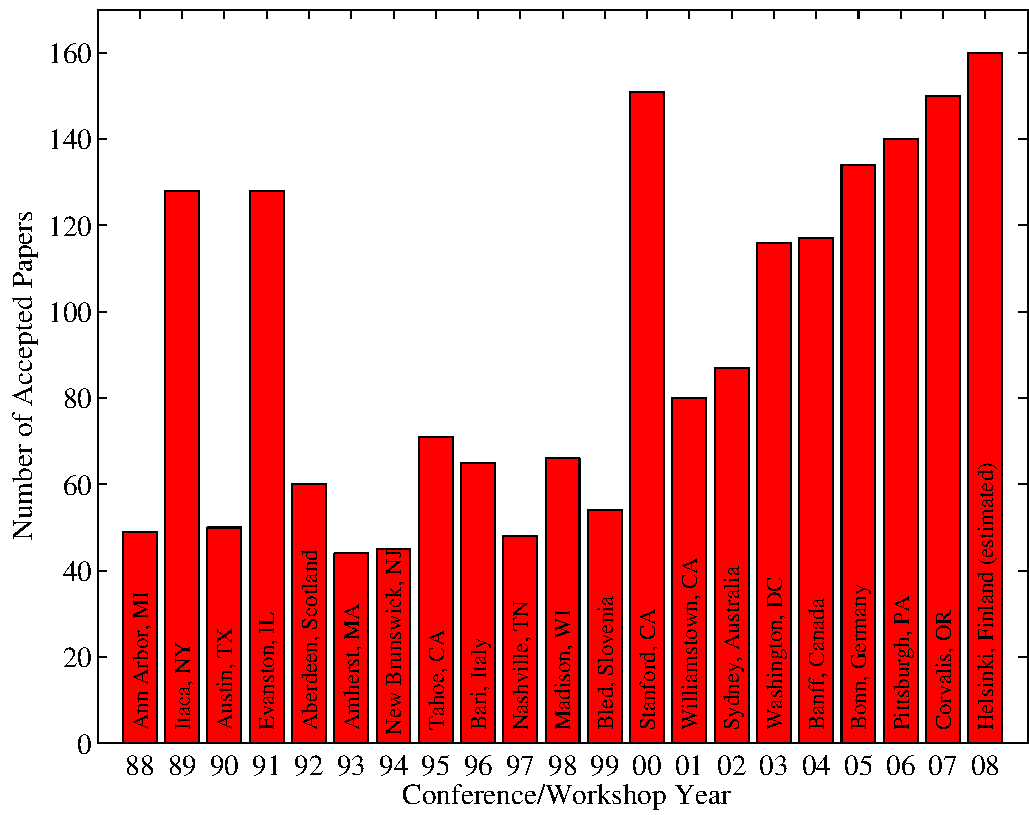
\includegraphics[width=\columnwidth]{icml_numpapers}}
\caption{Historical locations and number of accepted papers for International
Machine Learning Conferences (ICML 1993 -- ICML 2008) and International
Workshops on Machine Learning (ML 1988 -- ML 1992). At the time this figure was
produced, the number of accepted papers for ICML 2008 was unknown and instead
estimated.}
\label{icml-historical}
\end{center}
\vskip -0.2in
\end{figure}

\subsection{Figures}

You may want to include figures in the paper to illustrate
your approach and results. Such artwork should be centered,
legible, and separated from the text. Lines should be dark and at
least 0.5~points thick for purposes of reproduction, and text should
not appear on a gray background.

Label all distinct components of each figure. If the figure takes the
form of a graph, then give a name for each axis and include a legend
that briefly describes each curve. Do not include a title inside the
figure; instead, the caption should serve this function.

Number figures sequentially, placing the figure number and caption
\emph{after} the graphics, with at least 0.1~inches of space before
the caption and 0.1~inches after it, as in
\cref{icml-historical}. The figure caption should be set in
9~point type and centered unless it runs two or more lines, in which
case it should be flush left. You may float figures to the top or
bottom of a column, and you may set wide figures across both columns
(use the environment \texttt{figure*} in \LaTeX). Always place
two-column figures at the top or bottom of the page.

\subsection{Algorithms}

If you are using \LaTeX, please use the ``algorithm'' and ``algorithmic''
environments to format pseudocode. These require
the corresponding stylefiles, algorithm.sty and
algorithmic.sty, which are supplied with this package.
\cref{alg:example} shows an example.

\begin{algorithm}[tb]
   \caption{Bubble Sort}
   \label{alg:example}
\begin{algorithmic}
   \STATE {\bfseries Input:} data $x_i$, size $m$
   \REPEAT
   \STATE Initialize $noChange = true$.
   \FOR{$i=1$ {\bfseries to} $m-1$}
   \IF{$x_i > x_{i+1}$}
   \STATE Swap $x_i$ and $x_{i+1}$
   \STATE $noChange = false$
   \ENDIF
   \ENDFOR
   \UNTIL{$noChange$ is $true$}
\end{algorithmic}
\end{algorithm}

\subsection{Tables}

You may also want to include tables that summarize material. Like
figures, these should be centered, legible, and numbered consecutively.
However, place the title \emph{above} the table with at least
0.1~inches of space before the title and the same after it, as in
\cref{sample-table}. The table title should be set in 9~point
type and centered unless it runs two or more lines, in which case it
should be flush left.

% Note use of \abovespace and \belowspace to get reasonable spacing
% above and below tabular lines.


Tables contain textual material, whereas figures contain graphical material.
Specify the contents of each row and column in the table's topmost
row. Again, you may float tables to a column's top or bottom, and set
wide tables across both columns. Place two-column tables at the
top or bottom of the page.

\subsection{Theorems and such}
The preferred way is to number definitions, propositions, lemmas, etc. consecutively, within sections, as shown below.
\begin{definition}
\label{def:inj}
A function $f:X \to Y$ is injective if for any $x,y\in X$ different, $f(x)\ne f(y)$.
\end{definition}
Using \cref{def:inj} we immediate get the following result:
\begin{proposition}
If $f$ is injective mapping a set $X$ to another set $Y$, 
the cardinality of $Y$ is at least as large as that of $X$
\end{proposition}
\begin{proof} 
Left as an exercise to the reader. 
\end{proof}
\cref{lem:usefullemma} stated next will prove to be useful.
\begin{lemma}
\label{lem:usefullemma}
For any $f:X \to Y$ and $g:Y\to Z$ injective functions, $f \circ g$ is injective.
\end{lemma}
\begin{theorem}
\label{thm:bigtheorem}
If $f:X\to Y$ is bijective, the cardinality of $X$ and $Y$ are the same.
\end{theorem}
An easy corollary of \cref{thm:bigtheorem} is the following:
\begin{corollary}
If $f:X\to Y$ is bijective, 
the cardinality of $X$ is at least as large as that of $Y$.
\end{corollary}
\begin{assumption}
The set $X$ is finite.
\label{ass:xfinite}
\end{assumption}
\begin{remark}
According to some, it is only the finite case (cf. \cref{ass:xfinite}) that is interesting.
\end{remark}
%restatable

\subsection{Citations and References}

Please use APA reference format regardless of your formatter
or word processor. If you rely on the \LaTeX\/ bibliographic
facility, use \texttt{natbib.sty} and \texttt{icml2022.bst}
included in the style-file package to obtain this format.

Citations within the text should include the authors' last names and
year. If the authors' names are included in the sentence, place only
the year in parentheses, for example when referencing Arthur Samuel's
pioneering work \yrcite{Samuel59}. Otherwise place the entire
reference in parentheses with the authors and year separated by a
comma \cite{Samuel59}. List multiple references separated by
semicolons \cite{kearns89,Samuel59,mitchell80}. Use the `et~al.'
construct only for citations with three or more authors or after
listing all authors to a publication in an earlier reference \cite{MachineLearningI}.

Authors should cite their own work in the third person
in the initial version of their paper submitted for blind review.
Please refer to \cref{author info} for detailed instructions on how to
cite your own papers.

Use an unnumbered first-level section heading for the references, and use a
hanging indent style, with the first line of the reference flush against the
left margin and subsequent lines indented by 10 points. The references at the
end of this document give examples for journal articles \cite{Samuel59},
conference publications \cite{langley00}, book chapters \cite{Newell81}, books
\cite{DudaHart2nd}, edited volumes \cite{MachineLearningI}, technical reports
\cite{mitchell80}, and dissertations \cite{kearns89}.

Alphabetize references by the surnames of the first authors, with
single author entries preceding multiple author entries. Order
references for the same authors by year of publication, with the
earliest first. Make sure that each reference includes all relevant
information (e.g., page numbers).

Please put some effort into making references complete, presentable, and
consistent, e.g. use the actual current name of authors.
If using bibtex, please protect capital letters of names and
abbreviations in titles, for example, use \{B\}ayesian or \{L\}ipschitz
in your .bib file.

\section*{Accessibility}
Authors are kindly asked to make their submissions as accessible as possible for everyone including people with disabilities and sensory or neurological differences.
Tips of how to achieve this and what to pay attention to will be provided on the conference website \url{http://icml.cc/}.

\section*{Software and Data}

If a paper is accepted, we strongly encourage the publication of software and data with the
camera-ready version of the paper whenever appropriate. This can be
done by including a URL in the camera-ready copy. However, \textbf{do not}
include URLs that reveal your institution or identity in your
submission for review. Instead, provide an anonymous URL or upload
the material as ``Supplementary Material'' into the CMT reviewing
system. Note that reviewers are not required to look at this material
when writing their review.

% Acknowledgements should only appear in the accepted version.
\section*{Acknowledgements}

\textbf{Do not} include acknowledgements in the initial version of
the paper submitted for blind review.

If a paper is accepted, the final camera-ready version can (and
probably should) include acknowledgements. In this case, please
place such acknowledgements in an unnumbered section at the
end of the paper. Typically, this will include thanks to reviewers
who gave useful comments, to colleagues who contributed to the ideas,
and to funding agencies and corporate sponsors that provided financial
support.


% In the unusual situation where you want a paper to appear in the
% references without citing it in the main text, use \nocite
\nocite{langley00}

\bibliography{example_paper}
\bibliographystyle{icml2022}


%%%%%%%%%%%%%%%%%%%%%%%%%%%%%%%%%%%%%%%%%%%%%%%%%%%%%%%%%%%%%%%%%%%%%%%%%%%%%%%
%%%%%%%%%%%%%%%%%%%%%%%%%%%%%%%%%%%%%%%%%%%%%%%%%%%%%%%%%%%%%%%%%%%%%%%%%%%%%%%
% APPENDIX
%%%%%%%%%%%%%%%%%%%%%%%%%%%%%%%%%%%%%%%%%%%%%%%%%%%%%%%%%%%%%%%%%%%%%%%%%%%%%%%
%%%%%%%%%%%%%%%%%%%%%%%%%%%%%%%%%%%%%%%%%%%%%%%%%%%%%%%%%%%%%%%%%%%%%%%%%%%%%%%
\newpage
\appendix
\onecolumn
\section{You \emph{can} have an appendix here.}

You can have as much text here as you want. The main body must be at most $8$ pages long.
For the final version, one more page can be added.
If you want, you can use an appendix like this one, even using the one-column format.
%%%%%%%%%%%%%%%%%%%%%%%%%%%%%%%%%%%%%%%%%%%%%%%%%%%%%%%%%%%%%%%%%%%%%%%%%%%%%%%
%%%%%%%%%%%%%%%%%%%%%%%%%%%%%%%%%%%%%%%%%%%%%%%%%%%%%%%%%%%%%%%%%%%%%%%%%%%%%%%


\end{document}


% This document was modified from the file originally made available by
% Pat Langley and Andrea Danyluk for ICML-2K. This version was created
% by Iain Murray in 2018, and modified by Alexandre Bouchard in
% 2019 and 2021 and by Csaba Szepesvari, Gang Niu and Sivan Sabato in 2022. 
% Previous contributors include Dan Roy, Lise Getoor and Tobias
% Scheffer, which was slightly modified from the 2010 version by
% Thorsten Joachims & Johannes Fuernkranz, slightly modified from the
% 2009 version by Kiri Wagstaff and Sam Roweis's 2008 version, which is
% slightly modified from Prasad Tadepalli's 2007 version which is a
% lightly changed version of the previous year's version by Andrew
% Moore, which was in turn edited from those of Kristian Kersting and
% Codrina Lauth. Alex Smola contributed to the algorithmic style files.
